\documentclass[12pt]{article}
\usepackage[margin=1in]{geometry}
\usepackage{graphicx}
\usepackage{booktabs}
\usepackage{xcolor}
\usepackage{float}
\usepackage{hyperref}
\usepackage{amsmath}
\usepackage{setspace}

\hypersetup{
    colorlinks=true,
    linkcolor=blue!60!black,
    citecolor=blue!60!black,
    urlcolor=blue!60!black
}
\onehalfspacing

\title{
    \vspace{-1cm}
    \Large\textbf{Cookie Cats A/B Testing Analysis:\\
    Evaluating Gate Placement on Player Retention}
}
\author{
    William Chen
}
\date{}

\setlength{\parindent}{0pt}
\setlength{\parskip}{8pt}

\begin{document}

\maketitle
\thispagestyle{empty}

\begin{abstract}
This report presents an A/B testing analysis of the Cookie Cats mobile game, 
examining whether gate placement at level 30 (\textit{gate\_30}) versus level 40 
(\textit{gate\_40}) affects player retention across 90,189 players. Both Frequentist 
and Bayesian approaches are applied to binary retention metrics (\textit{retention\_1}, 
\textit{retention\_7}) and a continuous game rounds metric (\textit{sum\_gamerounds}).

Frequentist results show a statistically significant difference in 7-day retention 
($\chi^2(1) = 9.959$, $p = 0.0016$), while 1-day retention shows no significant 
difference ($p = 0.0755$). Bayesian posterior analysis confirms a 99.92\% probability 
that \textit{gate\_30} yields higher 7-day retention, with an estimated advantage 
of 0.31\%--1.33\%. All effect sizes remain negligible, though the consistency across 
both methods supports retaining the gate at level 30.
\end{abstract}

\newpage

% ══════════════════════════════════════════════════════════
\section{Introduction}
% ══════════════════════════════════════════════════════════

Player retention is a critical metric in the mobile gaming industry, as retaining 
existing players is substantially more cost-effective than acquiring new ones. 
This report presents an A/B testing analysis of the Cookie Cats mobile game, 
examining whether gate placement at level 30 (\textit{gate\_30}) versus level 40 
(\textit{gate\_40}) affects player retention.

The dataset contains both binary outcomes (\textit{retention\_1}, \textit{retention\_7}) 
and a continuous metric (\textit{sum\_gamerounds}), requiring different statistical 
approaches. A Frequentist analysis is first applied, using the Chi-square test for 
binary outcomes and the Mann-Whitney U test for the right-skewed continuous metric. 
While Frequentist testing confirms whether a difference is statistically significant, 
it cannot quantify how probable that difference is. A Bayesian approach is therefore 
applied using conjugate models to provide posterior probabilities and credible 
intervals for a more interpretable conclusion.

% ══════════════════════════════════════════════════════════
\section{Data}
% ══════════════════════════════════════════════════════════

\subsection{Dataset Overview}

The dataset contains 90,189 player records sourced from Kaggle, collected from a randomized 
A/B experiment conducted on the mobile puzzle game Cookie Cats. Players were randomly assigned 
to one of two experimental groups upon installation: \textit{gate\_30} (control, $n = 44{,}700$) 
and \textit{gate\_40} (treatment, $n = 45{,}489$). The two groups are well-balanced in size, 
with no missing values detected across all variables. The primary outcome variables are 
\textit{retention\_1} and \textit{retention\_7}, both binary indicators representing whether 
a player returned to the game 1 day and 7 days after installation, respectively.

\subsection{Feature Description}

The dataset contains 5 variables: 1 identifier (\textit{userid}, excluded from analysis), 
1 grouping variable (\textit{version}), 1 behavioral metric (\textit{sum\_gamerounds}), 
and 2 binary outcome variables (\textit{retention\_1}, \textit{retention\_7}). 
\textit{version} indicates the experimental group assigned to each player, either 
\textit{gate\_30} (control) or \textit{gate\_40} (treatment). \textit{sum\_gamerounds} 
records the total number of game rounds played within the first 14 days after installation. 
\textit{retention\_1} and \textit{retention\_7} are logical variables indicating whether 
a player returned to the game 1 day and 7 days after installation, respectively.

% ══════════════════════════════════════════════════════════
\section{Exploratory Data Analysis}
% ══════════════════════════════════════════════════════════

\subsection{Summary Statistics}

The dataset contains 90,189 complete observations with no missing values detected. 
\textit{sum\_gamerounds} ranges from 0 to 49,854 with a mean of 51.87 and a median 
of 16, indicating a heavily right-skewed distribution. The two experimental groups 
are well-balanced: \textit{gate\_30} contains 44,700 players (49.6\%) and 
\textit{gate\_40} contains 45,489 players (50.4\%). Overall 1-day retention rate 
is 44.5\% and 7-day retention rate is 18.6\%.

\subsection{Feature Distribution by Version}

Figure~\ref{fig:retention_bar} shows the retention rates for both experimental groups. 
\textit{gate\_30} and \textit{gate\_40} show similar 1-day retention rates (approximately 
44.8\% vs.\ 44.2\%), while \textit{gate\_30} shows a slightly higher 7-day retention rate 
(19.0\% vs.\ 18.2\%).

\begin{figure}[H]
    \centering
    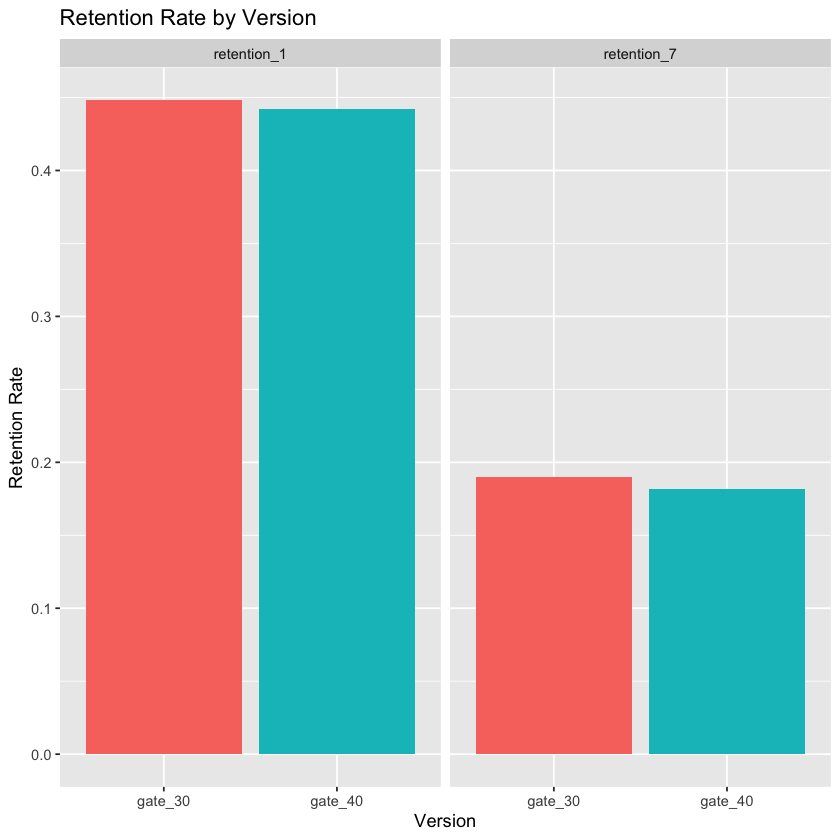
\includegraphics[width=0.55\textwidth]{figures/retention_bar.png}
    \caption{Retention Rate by Version}
    \label{fig:retention_bar}
\end{figure}

\subsection{Outlier Detection}

To assess the presence of extreme values in \textit{sum\_gamerounds}, the IQR method 
was applied. Figure~\ref{fig:gamerounds_boxplot} visualizes the IQR $\times$ 3 
outlier threshold across both groups on a log scale. A total of 5,704 observations 
(6.32\%) exceed the upper bound. Since \textit{sum\_gamerounds} is a secondary 
metric and the definition of a game round is ambiguous, outliers are retained in 
the analysis.

\begin{figure}[H]
    \centering
    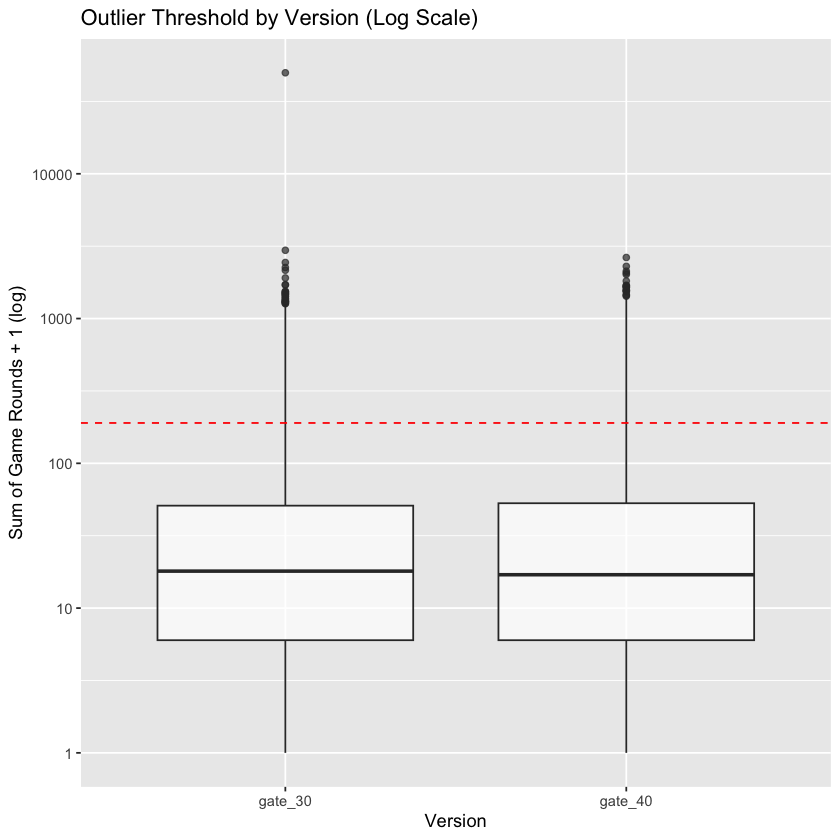
\includegraphics[width=0.6\textwidth]{figures/gamerounds_boxplot.png}
    \caption{Game Rounds by Version (Log Scale). The dashed red line indicates the IQR $\times$ 3 outlier threshold.}
    \label{fig:gamerounds_boxplot}
\end{figure}

% ══════════════════════════════════════════════════════════
\section{Methodology}
% ══════════════════════════════════════════════════════════

\subsection{Frequentist Approach}

\paragraph{Chi-Square Test}
The Chi-square test of independence was applied to evaluate whether gate placement 
is associated with binary retention outcomes (\textit{retention\_1}, \textit{retention\_7}). 
The null hypothesis states that retention is independent of version assignment.

\paragraph{Mann-Whitney U Test}
The Mann-Whitney U test was applied to compare \textit{sum\_gamerounds} between 
the two groups. As a non-parametric test, it does not assume normality and is 
therefore appropriate for skewed count data.

\subsection{Bayesian Approach}

\paragraph{Beta-Binomial Model}
For binary retention outcomes, a Beta-Binomial conjugate model was applied with 
an uninformative prior $\text{Beta}(1, 1)$, yielding the posterior:
\[
p \mid \text{data} \sim \text{Beta}(\alpha + \text{successes},\ \beta + \text{failures})
\]

\paragraph{Gamma-Poisson Model}
For \textit{sum\_gamerounds}, a Gamma-Poisson conjugate model was applied with 
prior $\text{Gamma}(1, 1)$, yielding the posterior:
\[
\lambda \mid \text{data} \sim \text{Gamma}\!\left(\alpha + \sum x_i,\ \beta + n\right)
\]

\subsection{Evaluation Metrics}

Frequentist tests are evaluated using p-value and effect size: Cramér's $V$ for 
Chi-square tests and rank-biserial $r$ for the Mann-Whitney U test.

For Bayesian models, Monte Carlo sampling ($n = 100{,}000$) was used to estimate 
the following metrics:

\begin{itemize}
    \item $P(\textit{gate\_30} > \textit{gate\_40})$: posterior probability that \textit{gate\_30} outperforms \textit{gate\_40}
    \item \textbf{95\% Credible Interval}: the range of plausible differences with 95\% posterior probability
\end{itemize}

% ══════════════════════════════════════════════════════════
\section{Results}
% ══════════════════════════════════════════════════════════

\subsection{Frequentist Results}

Table~\ref{tab:chisq} presents the Chi-square test results for both retention metrics. 
\textit{retention\_7} shows a statistically significant association with gate placement 
($\chi^2(1) = 9.959$, $p = 0.0016$), while \textit{retention\_1} does not reach 
significance ($\chi^2(1) = 3.159$, $p = 0.0755$). However, both Cramér's $V$ values 
are below 0.02, indicating a negligible practical effect.

\begin{table}[H]
\centering
\begin{tabular}{lrrrr}
\toprule
\textbf{Metric} & \textbf{$\chi^2$} & \textbf{df} & \textbf{p-value} & \textbf{Cramér's $V$} \\
\midrule
\textit{retention\_1} & 3.159 & 1 & 0.0755 & 0.0059 \\
\textit{retention\_7} & 9.959 & 1 & 0.0016 & 0.0105 \\
\bottomrule
\end{tabular}
\caption{Chi-square test results for retention metrics}
\label{tab:chisq}
\end{table}

Figures~\ref{fig:ci_r1} and~\ref{fig:ci_r7} show the retention rates with 95\% 
confidence intervals for each group. For \textit{retention\_1}, \textit{gate\_30} 
achieves 44.8\% and \textit{gate\_40} achieves 44.2\%, with overlapping intervals 
indicating no reliable difference. For \textit{retention\_7}, \textit{gate\_30} 
achieves 19.0\% and \textit{gate\_40} achieves 18.2\%, with non-overlapping intervals 
confirming a statistically significant difference.

\begin{figure}[H]
    \centering
    \begin{minipage}{0.48\textwidth}
        \centering
        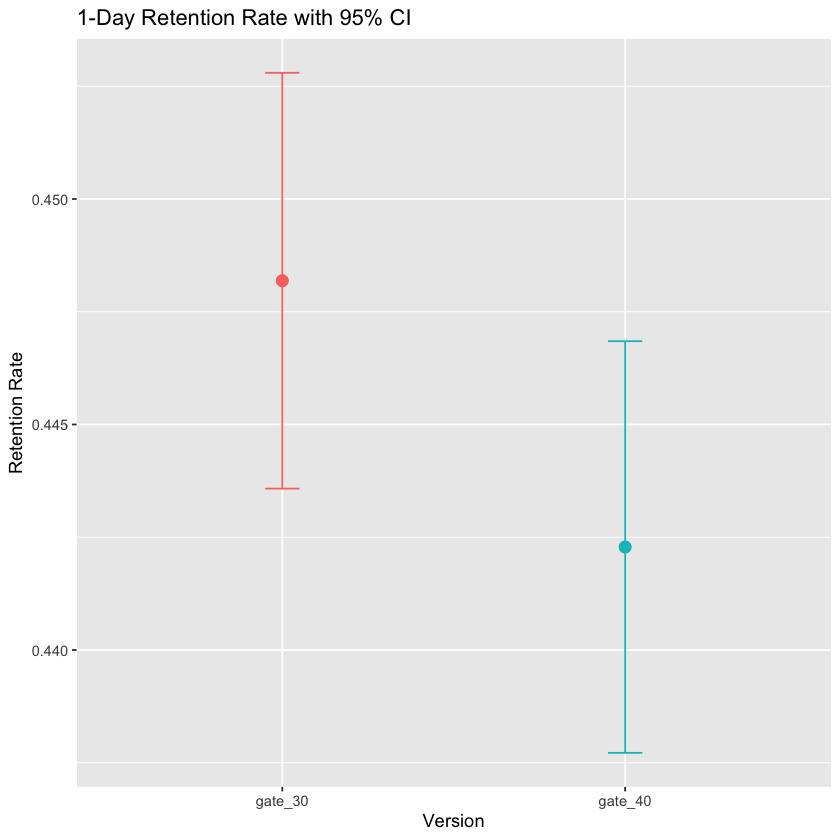
\includegraphics[width=\textwidth]{figures/retention_ci_r1.png}
        \caption{1-Day Retention Rate (95\% CI)}
        \label{fig:ci_r1}
    \end{minipage}
    \hfill
    \begin{minipage}{0.48\textwidth}
        \centering
        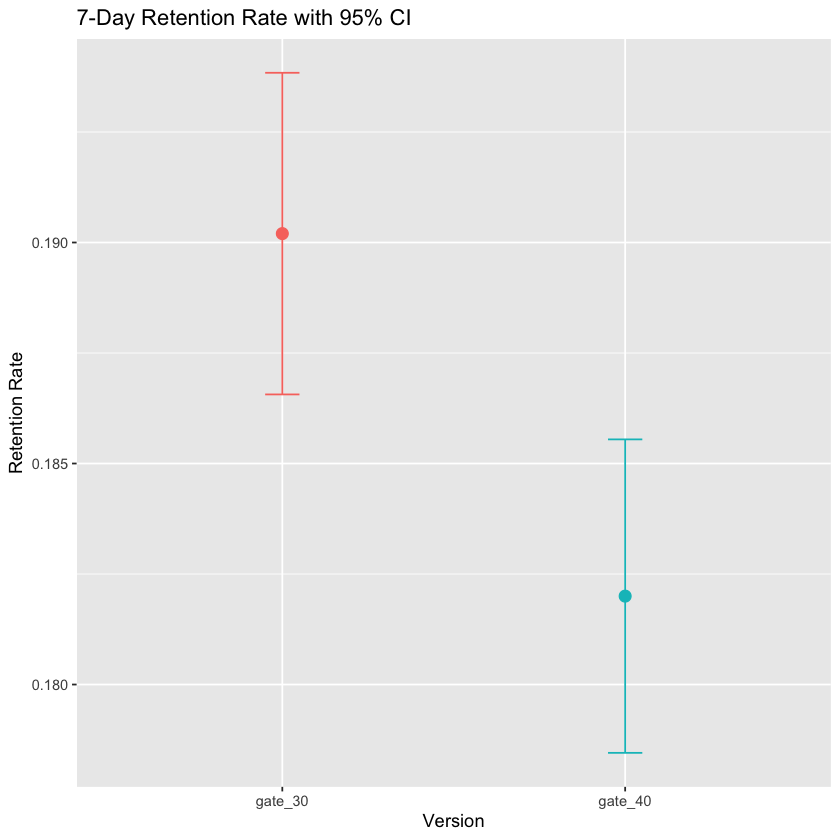
\includegraphics[width=\textwidth]{figures/retention_ci_r7.png}
        \caption{7-Day Retention Rate (95\% CI)}
        \label{fig:ci_r7}
    \end{minipage}
\end{figure}

For \textit{sum\_gamerounds}, the Mann-Whitney U test yields $W = 1{,}024{,}331{,}250$, 
$p = 0.0502$, with a rank-biserial correlation of $r = -0.0075$, indicating no 
significant difference and a negligible effect size between the two groups.

\begin{table}[H]
\centering
\begin{tabular}{lrrr}
\toprule
\textbf{Metric} & \textbf{W} & \textbf{p-value} & \textbf{Rank-Biserial $r$} \\
\midrule
\textit{sum\_gamerounds} & 1{,}024{,}331{,}250 & 0.0502 & $-0.0075$ \\
\bottomrule
\end{tabular}
\caption{Mann-Whitney U test results for game rounds}
\label{tab:mw}
\end{table}

\subsection{Bayesian Results}

Table~\ref{tab:bayes} presents the Bayesian posterior results for all three metrics. 
For \textit{retention\_1}, the probability is 96.19\% with a credible interval of 
$[-0.0006, 0.0124]$, which includes zero, suggesting less certainty. 
For \textit{retention\_7}, there is a 99.92\% posterior probability that \textit{gate\_30} 
outperforms \textit{gate\_40}, with a 95\% credible interval of $[0.0031, 0.0133]$, 
indicating \textit{gate\_30} retains 0.31\%--1.33\% more players after 7 days. 
For \textit{sum\_gamerounds}, \textit{gate\_30} players accumulate on average 
1.06--1.25 more game rounds over the 14-day observation period with 100\% posterior probability.

\begin{table}[H]
\centering
\begin{tabular}{lrrr}
\toprule
\textbf{Metric} & \textbf{$P(\textit{gate\_30} > \textit{gate\_40})$} & \textbf{CI Lower} & \textbf{CI Upper} \\
\midrule
\textit{retention\_1}    & 96.19\% & $-0.0006$ & $0.0124$ \\
\textit{retention\_7}    & 99.92\% & $0.0031$  & $0.0133$ \\
\textit{sum\_gamerounds} & 100.00\% & $1.0631$  & $1.2519$ \\
\bottomrule
\end{tabular}
\caption{Bayesian posterior results}
\label{tab:bayes}
\end{table}

Figures~\ref{fig:posterior_r1} and~\ref{fig:posterior_r7} show the posterior 
distributions of the retention rates for both groups. The overlapping distributions 
in \textit{retention\_1} reflect greater uncertainty, while the narrow, well-separated 
distributions in \textit{retention\_7} confirm high certainty in the superiority 
of \textit{gate\_30}.

\begin{figure}[H]
    \centering
    \begin{minipage}{0.48\textwidth}
        \centering
        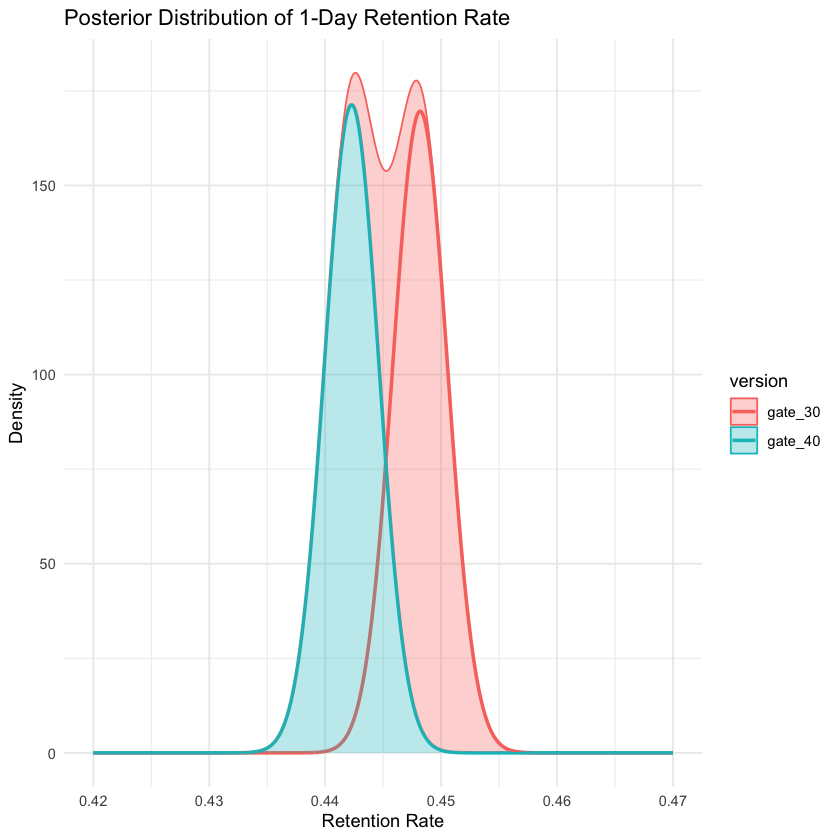
\includegraphics[width=\textwidth]{figures/posterior_r1.png}
        \caption{Posterior Distribution (1-Day)}
        \label{fig:posterior_r1}
    \end{minipage}
    \hfill
    \begin{minipage}{0.48\textwidth}
        \centering
        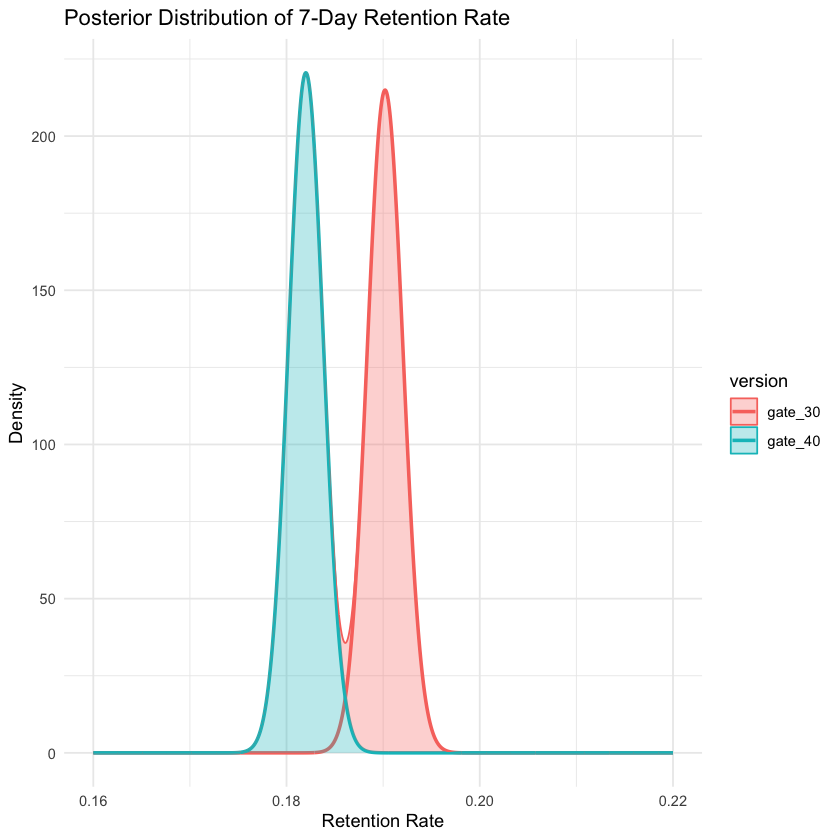
\includegraphics[width=\textwidth]{figures/posterior_r7.png}
        \caption{Posterior Distribution (7-Day)}
        \label{fig:posterior_r7}
    \end{minipage}
\end{figure}

Figure~\ref{fig:posterior_gp} shows the posterior distribution of the average game 
rounds rate under the Gamma-Poisson model. The two distributions are well-separated, 
reflecting high certainty that \textit{gate\_30} players play more rounds on average.

\begin{figure}[H]
    \centering
    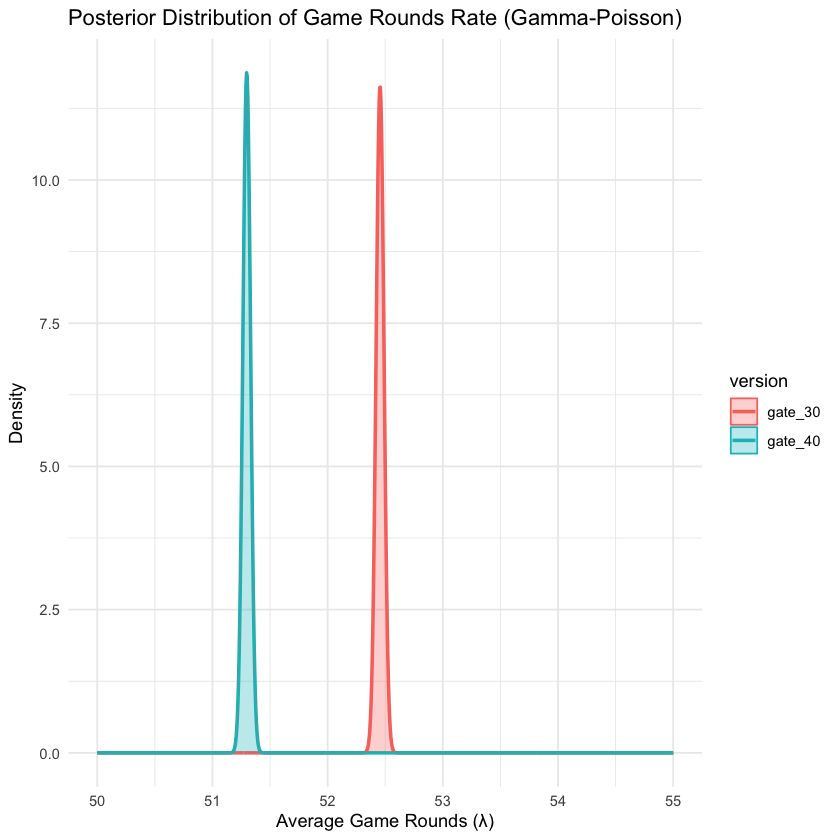
\includegraphics[width=0.6\textwidth]{figures/posterior_gp.png}
    \caption{Posterior Distribution of Game Rounds Rate (Gamma-Poisson)}
    \label{fig:posterior_gp}
\end{figure}

\subsection{Overall Comparison}

Both Frequentist and Bayesian approaches consistently indicate that \textit{gate\_30} 
outperforms \textit{gate\_40} across all three metrics. The Frequentist approach 
confirms a statistically significant difference in \textit{retention\_7} ($p = 0.0016$), 
while \textit{retention\_1} and \textit{sum\_gamerounds} do not reach significance. 
The Bayesian approach provides a more interpretable conclusion: \textit{gate\_30} is 
superior in 7-day retention with 99.92\% posterior probability, and all three metrics 
show posterior probabilities above 96\%. Notably, all effect sizes remain negligible, 
suggesting the practical impact is limited despite statistical significance.


% ══════════════════════════════════════════════════════════
\section{Discussion \& Conclusion}
% ══════════════════════════════════════════════════════════

\subsection{Key Findings}

Both Frequentist and Bayesian analyses consistently indicate that \textit{gate\_30} 
outperforms \textit{gate\_40}. The effect is most pronounced in \textit{retention\_7}, 
where both methods converge on the same conclusion with high certainty.

A notable observation is that \textit{retention\_1} shows no reliable difference 
between the two groups, suggesting that the gate placement effect takes time to 
manifest. Players are unlikely to have reached the gate within the first day, 
making 1-day retention an insufficient metric for evaluating gate effects.

Despite statistical significance in \textit{retention\_7}, all effect sizes remain 
negligible. This is a common pattern in large-sample A/B tests, where even trivial 
differences can reach significance.

\subsection{Business Recommendations}

Based on the analysis, \textbf{retaining the gate at level 30 is recommended}. 
Placing the gate earlier forces players to stop before reaching full satisfaction, 
leaving an unfinished desire that motivates them to return. This aligns with the 
theory of \textit{hedonic adaptation}: enforced breaks preserve the novelty of the 
game and sustain long-term engagement.

In contrast, \textit{gate\_40} allows players to play longer before being interrupted. 
By the time the gate appears, players have already experienced sufficient satisfaction, 
reducing their motivation to return. The result is a measurable decline in 7-day 
retention.

While the retention advantage of \textit{gate\_30} is statistically significant, 
the effect size remains small. At scale, however, even a marginal improvement in 
retention carries meaningful implications for revenue and player lifetime value.

\subsection{Limitations}

\subsubsection*{Dataset Limitations}
The definition of \textit{sum\_gamerounds} is ambiguous, as it is unclear whether 
one round corresponds to one level attempt or one completed level. This limits 
the interpretability of the Gamma-Poisson results and the outlier analysis. 
Additionally, the dataset does not include contextual variables such as player 
demographics, device type, or prior gaming experience, which may confound the 
relationship between gate placement and retention.

\subsubsection*{Evaluation Metrics}
The analysis relies solely on \textit{retention\_1} and \textit{retention\_7} as 
outcome metrics. While 7-day retention captures the gate effect more reliably, 
a single time point may not fully represent long-term player behavior. Furthermore, 
the confidence interval plots suggest that the observed differences, while 
statistically detectable, are narrow in practical terms. Additional metrics such 
as 14-day or 30-day retention, or revenue per player, could provide a more 
comprehensive evaluation.

\begin{thebibliography}{9}

\bibitem{cookiecats}
Mobile Games (2024).
\textit{Cookie Cats} [Dataset].
Kaggle.
\texttt{https://www.kaggle.com/datasets/yufengsui/mobile-games-ab-testing}

\end{thebibliography}

\end{document}
